% Options for packages loaded elsewhere
\PassOptionsToPackage{unicode}{hyperref}
\PassOptionsToPackage{hyphens}{url}
\PassOptionsToPackage{dvipsnames,svgnames,x11names}{xcolor}
%
\documentclass[
  a4paper,
  noprof,
  12pt,
  notoc,
  nosols,
  nobib]{mnye}

\usepackage{amsmath,amssymb}
\usepackage{iftex}
\ifPDFTeX
  \usepackage[T1]{fontenc}
  \usepackage[utf8]{inputenc}
  \usepackage{textcomp} % provide euro and other symbols
\else % if luatex or xetex
  \usepackage{unicode-math}
  \defaultfontfeatures{Scale=MatchLowercase}
  \defaultfontfeatures[\rmfamily]{Ligatures=TeX,Scale=1}
\fi
\usepackage{lmodern}
\ifPDFTeX\else  
    % xetex/luatex font selection
\fi
% Use upquote if available, for straight quotes in verbatim environments
\IfFileExists{upquote.sty}{\usepackage{upquote}}{}
\IfFileExists{microtype.sty}{% use microtype if available
  \usepackage[]{microtype}
  \UseMicrotypeSet[protrusion]{basicmath} % disable protrusion for tt fonts
}{}
\makeatletter
\@ifundefined{KOMAClassName}{% if non-KOMA class
  \IfFileExists{parskip.sty}{%
    \usepackage{parskip}
  }{% else
    \setlength{\parindent}{0pt}
    \setlength{\parskip}{6pt plus 2pt minus 1pt}}
}{% if KOMA class
  \KOMAoptions{parskip=half}}
\makeatother
\usepackage{xcolor}
\setlength{\emergencystretch}{3em} % prevent overfull lines
\setcounter{secnumdepth}{5}
% Make \paragraph and \subparagraph free-standing
\ifx\paragraph\undefined\else
  \let\oldparagraph\paragraph
  \renewcommand{\paragraph}[1]{\oldparagraph{#1}\mbox{}}
\fi
\ifx\subparagraph\undefined\else
  \let\oldsubparagraph\subparagraph
  \renewcommand{\subparagraph}[1]{\oldsubparagraph{#1}\mbox{}}
\fi

\usepackage{color}
\usepackage{fancyvrb}
\newcommand{\VerbBar}{|}
\newcommand{\VERB}{\Verb[commandchars=\\\{\}]}
\DefineVerbatimEnvironment{Highlighting}{Verbatim}{commandchars=\\\{\}}
% Add ',fontsize=\small' for more characters per line
\usepackage{framed}
\definecolor{shadecolor}{RGB}{241,243,245}
\newenvironment{Shaded}{\begin{snugshade}}{\end{snugshade}}
\newcommand{\AlertTok}[1]{\textcolor[rgb]{0.68,0.00,0.00}{#1}}
\newcommand{\AnnotationTok}[1]{\textcolor[rgb]{0.37,0.37,0.37}{#1}}
\newcommand{\AttributeTok}[1]{\textcolor[rgb]{0.40,0.45,0.13}{#1}}
\newcommand{\BaseNTok}[1]{\textcolor[rgb]{0.68,0.00,0.00}{#1}}
\newcommand{\BuiltInTok}[1]{\textcolor[rgb]{0.00,0.23,0.31}{#1}}
\newcommand{\CharTok}[1]{\textcolor[rgb]{0.13,0.47,0.30}{#1}}
\newcommand{\CommentTok}[1]{\textcolor[rgb]{0.37,0.37,0.37}{#1}}
\newcommand{\CommentVarTok}[1]{\textcolor[rgb]{0.37,0.37,0.37}{\textit{#1}}}
\newcommand{\ConstantTok}[1]{\textcolor[rgb]{0.56,0.35,0.01}{#1}}
\newcommand{\ControlFlowTok}[1]{\textcolor[rgb]{0.00,0.23,0.31}{#1}}
\newcommand{\DataTypeTok}[1]{\textcolor[rgb]{0.68,0.00,0.00}{#1}}
\newcommand{\DecValTok}[1]{\textcolor[rgb]{0.68,0.00,0.00}{#1}}
\newcommand{\DocumentationTok}[1]{\textcolor[rgb]{0.37,0.37,0.37}{\textit{#1}}}
\newcommand{\ErrorTok}[1]{\textcolor[rgb]{0.68,0.00,0.00}{#1}}
\newcommand{\ExtensionTok}[1]{\textcolor[rgb]{0.00,0.23,0.31}{#1}}
\newcommand{\FloatTok}[1]{\textcolor[rgb]{0.68,0.00,0.00}{#1}}
\newcommand{\FunctionTok}[1]{\textcolor[rgb]{0.28,0.35,0.67}{#1}}
\newcommand{\ImportTok}[1]{\textcolor[rgb]{0.00,0.46,0.62}{#1}}
\newcommand{\InformationTok}[1]{\textcolor[rgb]{0.37,0.37,0.37}{#1}}
\newcommand{\KeywordTok}[1]{\textcolor[rgb]{0.00,0.23,0.31}{#1}}
\newcommand{\NormalTok}[1]{\textcolor[rgb]{0.00,0.23,0.31}{#1}}
\newcommand{\OperatorTok}[1]{\textcolor[rgb]{0.37,0.37,0.37}{#1}}
\newcommand{\OtherTok}[1]{\textcolor[rgb]{0.00,0.23,0.31}{#1}}
\newcommand{\PreprocessorTok}[1]{\textcolor[rgb]{0.68,0.00,0.00}{#1}}
\newcommand{\RegionMarkerTok}[1]{\textcolor[rgb]{0.00,0.23,0.31}{#1}}
\newcommand{\SpecialCharTok}[1]{\textcolor[rgb]{0.37,0.37,0.37}{#1}}
\newcommand{\SpecialStringTok}[1]{\textcolor[rgb]{0.13,0.47,0.30}{#1}}
\newcommand{\StringTok}[1]{\textcolor[rgb]{0.13,0.47,0.30}{#1}}
\newcommand{\VariableTok}[1]{\textcolor[rgb]{0.07,0.07,0.07}{#1}}
\newcommand{\VerbatimStringTok}[1]{\textcolor[rgb]{0.13,0.47,0.30}{#1}}
\newcommand{\WarningTok}[1]{\textcolor[rgb]{0.37,0.37,0.37}{\textit{#1}}}

\providecommand{\tightlist}{%
  \setlength{\itemsep}{0pt}\setlength{\parskip}{0pt}}\usepackage{longtable,booktabs,array}
\usepackage{calc} % for calculating minipage widths
% Correct order of tables after \paragraph or \subparagraph
\usepackage{etoolbox}
\makeatletter
\patchcmd\longtable{\par}{\if@noskipsec\mbox{}\fi\par}{}{}
\makeatother
% Allow footnotes in longtable head/foot
\IfFileExists{footnotehyper.sty}{\usepackage{footnotehyper}}{\usepackage{footnote}}
\makesavenoteenv{longtable}
\usepackage{graphicx}
\makeatletter
\def\maxwidth{\ifdim\Gin@nat@width>\linewidth\linewidth\else\Gin@nat@width\fi}
\def\maxheight{\ifdim\Gin@nat@height>\textheight\textheight\else\Gin@nat@height\fi}
\makeatother
% Scale images if necessary, so that they will not overflow the page
% margins by default, and it is still possible to overwrite the defaults
% using explicit options in \includegraphics[width, height, ...]{}
\setkeys{Gin}{width=\maxwidth,height=\maxheight,keepaspectratio}
% Set default figure placement to htbp
\makeatletter
\def\fps@figure{htbp}
\makeatother

\usepackage{ehyperref}


\AtBeginDocument{
    \ifcsname c@theorem\endcsname % el contador theorem no está definido hasta que no se usa :::{#thm-label}
        \counterwithout{theorem}{section}
    \fi
    % \counterwithout{exercise}{section}
}

\AtBeginDocument{

    % Los entornos de teoremas que crea Quarto no están definidos hasta que no se usan.
    % Por ejemplo, exercise no está definido hasta que no se usa :::{#exr-label}

    % definition
    \ifcsname enddefinition\endcsname 
    \renewenvironment{definition}[1][]{
        \if\relax\detokenize{#1}\relax
            \dfn
        \else
            \dfn[note={#1}]
        \fi
    }{\enddfn}
    \fi

    % theorem
    \ifcsname endtheorem\endcsname 
    \renewenvironment{theorem}[1][]{%
        \if\relax\detokenize{#1}\relax%
            \thm%
        \else%
            \thm[note={#1}]%
        \fi%
        \unskip\unskip\ignorespaces
    }{\endthm}
    \fi   
    
    

    % example
    \ifcsname endexample\endcsname %
        \renewenvironment{example}[1][]{
            \if\relax\detokenize{#1}\relax
                \exmp
            \else
                \exmp[note={#1}]
            \fi
        }{\endex}
    \fi

    % exercise
    \ifcsname endexercise\endcsname %
        \renewenvironment{exercise}[1][]{
            \if\relax\detokenize{#1}\relax
                \ex
            \else
                \ex[note={#1}]
            \fi
        }{\endex}
    \fi

    % solution
    \ifcsname endsolution\endcsname 
        \renewenvironment{solution}{
                \sol
        }{\endsol}
    \fi
}
\graphicspath{{docs/}{./}}
\usepackage{fvextra}
\DefineVerbatimEnvironment{Highlighting}{Verbatim}{breaklines,commandchars=\\\{\}}
\usepackage{multido}
\tikzexternaldisable
\makeatletter
\makeatother
\makeatletter
\@ifpackageloaded{bookmark}{}{\usepackage{bookmark}}
\makeatother
\makeatletter
\@ifpackageloaded{caption}{}{\usepackage{caption}}
\AtBeginDocument{%
\ifdefined\contentsname
  \renewcommand*\contentsname{Tabla de contenidos}
\else
  \newcommand\contentsname{Tabla de contenidos}
\fi
\ifdefined\listfigurename
  \renewcommand*\listfigurename{Listado de Figuras}
\else
  \newcommand\listfigurename{Listado de Figuras}
\fi
\ifdefined\listtablename
  \renewcommand*\listtablename{Listado de Tablas}
\else
  \newcommand\listtablename{Listado de Tablas}
\fi
\ifdefined\figurename
  \renewcommand*\figurename{Figura}
\else
  \newcommand\figurename{Figura}
\fi
\ifdefined\tablename
  \renewcommand*\tablename{Tabla}
\else
  \newcommand\tablename{Tabla}
\fi
}
\@ifpackageloaded{float}{}{\usepackage{float}}
\floatstyle{ruled}
\@ifundefined{c@chapter}{\newfloat{codelisting}{h}{lop}}{\newfloat{codelisting}{h}{lop}[chapter]}
\floatname{codelisting}{Listado}
\newcommand*\listoflistings{\listof{codelisting}{Listado de Listados}}
\usepackage{amsthm}
\theoremstyle{definition}
\newtheorem{exercise}{Ejercicio}[section]
\theoremstyle{remark}
\AtBeginDocument{\renewcommand*{\proofname}{Prueba}}
\newtheorem*{remark}{Observación}
\newtheorem*{solution}{Solución}
\makeatother
\makeatletter
\@ifpackageloaded{caption}{}{\usepackage{caption}}
\@ifpackageloaded{subcaption}{}{\usepackage{subcaption}}
\makeatother
\makeatletter
\@ifpackageloaded{tcolorbox}{}{\usepackage[skins,breakable]{tcolorbox}}
\makeatother
\makeatletter
\@ifundefined{shadecolor}{\definecolor{shadecolor}{rgb}{.97, .97, .97}}
\makeatother
\makeatletter
\makeatother
\makeatletter
\makeatother
\ifLuaTeX
\usepackage[bidi=basic]{babel}
\else
\usepackage[bidi=default]{babel}
\fi
\babelprovide[main,import]{spanish}
% get rid of language-specific shorthands (see #6817):
\let\LanguageShortHands\languageshorthands
\def\languageshorthands#1{}
\ifLuaTeX
  \usepackage{selnolig}  % disable illegal ligatures
\fi
\usepackage[backend=biber]{biblatex}
\addbibresource{references.bib}
\IfFileExists{bookmark.sty}{\usepackage{bookmark}}{\usepackage{hyperref}}
\IfFileExists{xurl.sty}{\usepackage{xurl}}{} % add URL line breaks if available
\urlstyle{same} % disable monospaced font for URLs
\hypersetup{
  pdftitle={Exploración y visualización de datos con Python},
  pdfauthor={Eva María Mazcuñán Navarro},
  pdflang={es},
  colorlinks=true,
  linkcolor={elinkcolor},
  filecolor={Maroon},
  citecolor={ecitecolor},
  urlcolor={eurlcolor},
  pdfcreator={LaTeX via pandoc}}

\title{Exploración y visualización de datos con Python}
\term{2022-2023}
\degree{Grado en Ingeniería Informática / Mecánica}
\author{Eva María Mazcuñán Navarro}
\date{}

\begin{document}
\maketitle
\ifdefined\Shaded\renewenvironment{Shaded}{\begin{tcolorbox}[enhanced, frame hidden, boxrule=0pt, interior hidden, borderline west={3pt}{0pt}{shadecolor}, breakable, sharp corners]}{\end{tcolorbox}}\fi

\renewcommand*\contentsname{Contenidos}
{
\hypersetup{linkcolor=elinkcolor}
\pagenumbering{roman}%
\pagestyle{plain}%
\setcounter{tocdepth}{2}
\tableofcontents
\cleardoublepage{
\pagenumbering{arabic}%
\pagestyle{main}}
}
\bookmarksetup{startatroot}



\bookmarksetup{startatroot}

\hypertarget{sec-intro}{%
\section*{Introducción}\label{sec-intro}}
\addcontentsline{toc}{section}{Introducción}


En esta práctica aprenderás las técnicas básicas para explorar un
conjunto de datos con Python.

\hypertarget{los-pinguxfcinos-del-archipiuxe9lago-palmer}{%
\subsection*{Los pingüinos del archipiélago
Palmer}\label{los-pinguxfcinos-del-archipiuxe9lago-palmer}}
\addcontentsline{toc}{subsection}{Los pingüinos del archipiélago Palmer}

\markright{Los pingüinos del archipiélago Palmer}

Presentaremos las diferentes técnicas a través de ejemplos trabajando
con un conjunto de datos relativos a características morfológicas de
tres especies de pingüinos del archipiélago Palmer en la Antártida.

\begin{figure}[tbph]

{\centering 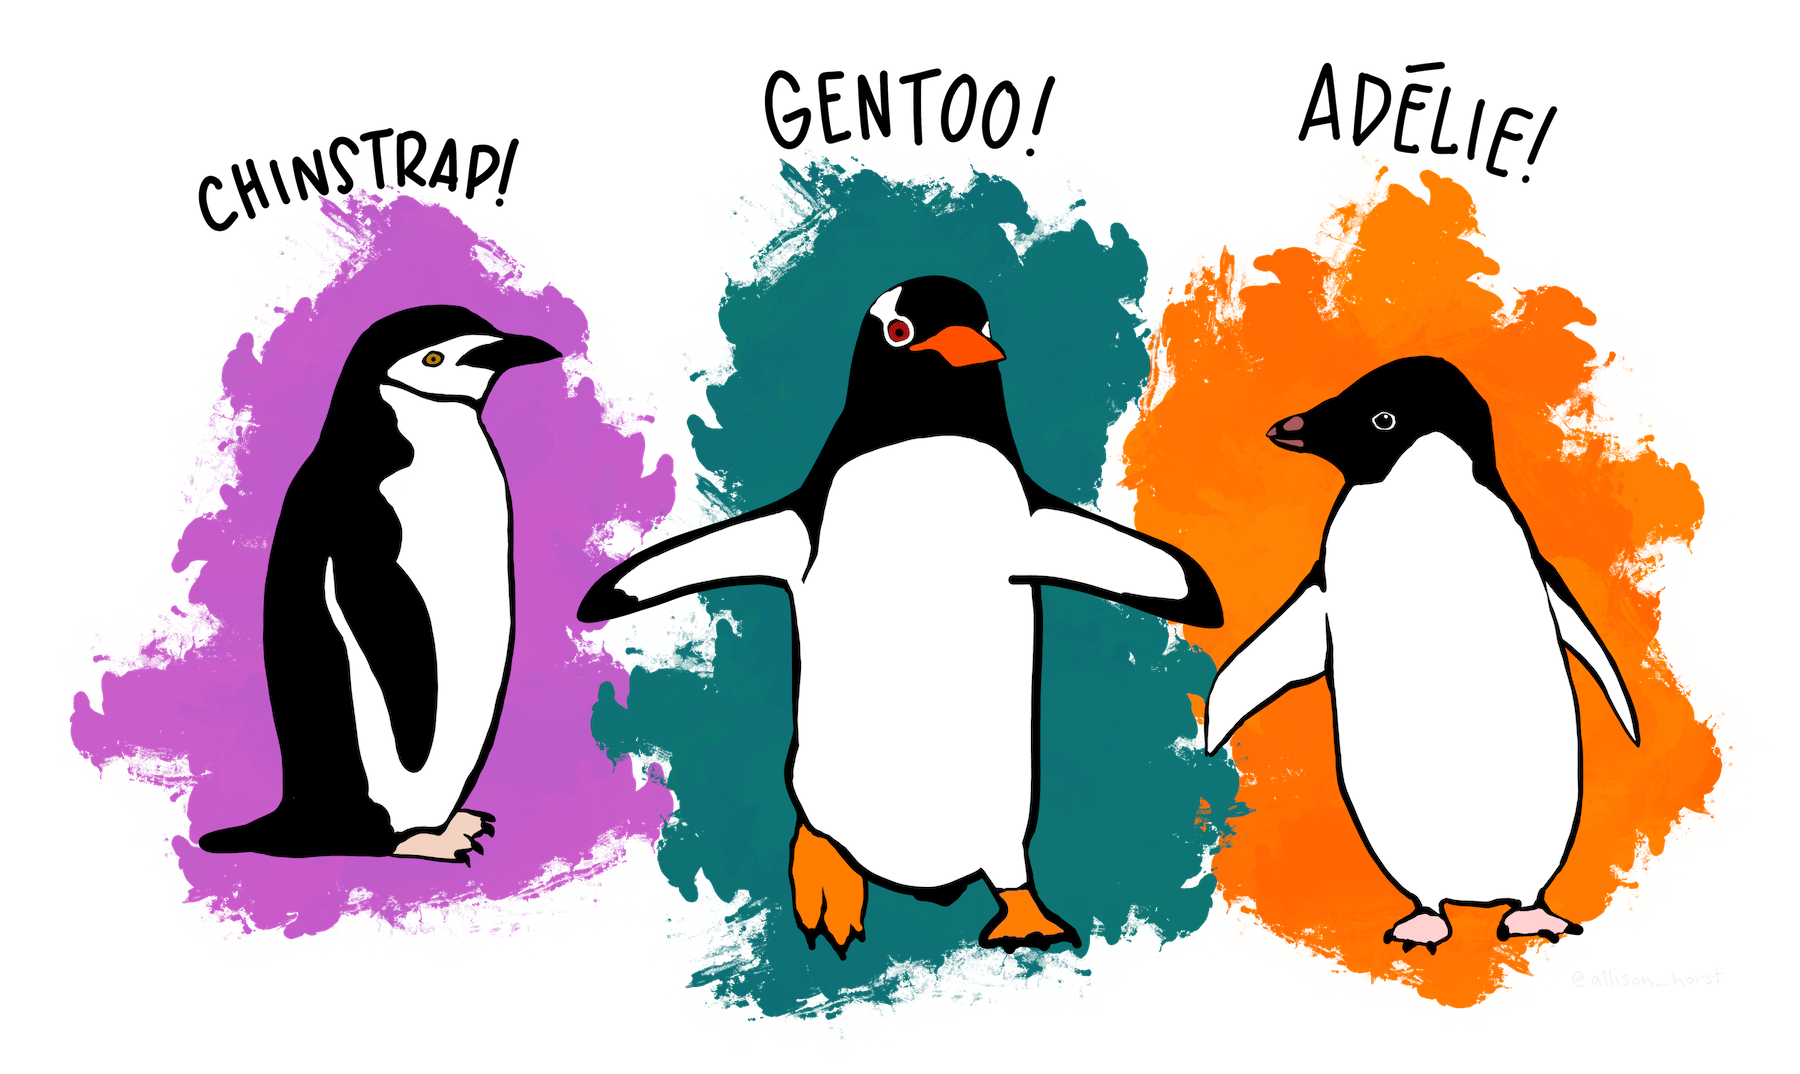
\includegraphics[width=0.8\textwidth,height=\textheight]{chapters/../img/penguins.png}

}

\caption{Ilustración de las tres especies de pingüinos del archipiélago
Palmer (Artista @allison\_horst)}

\end{figure}

Los datos fueron originalmente publicados en \textcite{Gorman2014}. Este
conjunto de datos se hizo popular a partir de la creación del paquete
\href{https://github.com/allisonhorst/palmerpenguins}{palmerpenguins} de
\href{https://www.r-project.org/}{R}. Hoy en día los datos de los
pingüinos del archipiélago Palmer se usan de forma extendida para
ilustrar las técnicas de exploración y visualización de datos no solo en
R, sino en muchos otros lenguajes de programación para estadística y
ciencia de datos, como Python. Nosotros accederemos a los datos a través
de
\href{https://github.com/mwaskom/seaborn-data/blob/master/penguins.csv}{este
enlace}, que proporciona los datos en formato CSV (\emph{comma separated
values}).

\hypertarget{objetivos}{%
\subsection*{Objetivos}\label{objetivos}}
\addcontentsline{toc}{subsection}{Objetivos}

\markright{Objetivos}

Aprenderás en concreto a calcular las medidas descriptivas más
representativas de las características de interés y a crear diferentes
tipos de gráficos o visualizaciones.

\begin{itemize}
\tightlist
\item[$\square$]
  Añadir un ejemplo de tabla y un ejemplo de gráfico. Por ejemplo, peso
  por especies.
\end{itemize}

\bookmarksetup{startatroot}

\hypertarget{libreruxedas}{%
\section{Librerías}\label{libreruxedas}}

\begin{Shaded}
\begin{Highlighting}[]
\ImportTok{import}\NormalTok{ pandas }\ImportTok{as}\NormalTok{ pd}
\ImportTok{import}\NormalTok{ numpy }\ImportTok{as}\NormalTok{ np}
\end{Highlighting}
\end{Shaded}

\hypertarget{pandas}{%
\subsection{\texorpdfstring{\texttt{pandas}}{pandas}}\label{pandas}}

\hypertarget{sub}{%
\subsubsection{sub}\label{sub}}

\begin{figure}[tbph]

{\centering 
\includegraphics[width=\textwidth,height=5em]{chapters/../img/pandas.png}

}

\end{figure}

\begin{figure}[tbph]

{\centering 
\includegraphics[width=\textwidth,height=5em]{chapters/../img/pandas.png}

}

\end{figure}

\hypertarget{numpy}{%
\subsection{\texorpdfstring{\texttt{numpy}}{numpy}}\label{numpy}}

\bookmarksetup{startatroot}

\hypertarget{datos}{%
\section{Datos}\label{datos}}

En esta sección importarás los datos sobre los pingüinos del
archipiélago Palmer presentados en la introducción y conocerás la
información que contienen.

\hypertarget{importar-los-datos}{%
\subsection{Importar los datos}\label{importar-los-datos}}

Como se indicó en la introducción, los datos con los que vamos a
trabajar están disponibles en la web en un fichero de formato
\texttt{CSV}.

Ejecuta las instrucciones a continuación para importar el archivo usando
la función \texttt{read\_csv()} y guardar el resultado en una variable
de nombre \texttt{penguins}:

\begin{Shaded}
\begin{Highlighting}[]
\NormalTok{url }\OperatorTok{=} \StringTok{"https://raw.githubusercontent.com/mwaskom/seaborn{-}data/master/penguins.csv"}
\NormalTok{penguins }\OperatorTok{=}\NormalTok{ pd.read\_csv(url)}
\end{Highlighting}
\end{Shaded}

El objeto \texttt{penguins} que acabas de crear es una \textbf{hoja de
datos}, representada en \texttt{pandas} con la clase \texttt{DataFrame}.

En los siguientes apartados aprenderás a realizar una exploración
inicial de la hoja de datos \texttt{penguins} que acabas de crear para
conocer su estructura y la información que contiene.

\hypertarget{dimensiones}{%
\subsection{Dimensiones}\label{dimensiones}}

Una hoja de datos es una estructura matricial o tabular que contiene
datos organizados por filas y columnas.

Para saber las dimensiones de nuestra hoja de datos \texttt{penguins}
consulta su propiedad \texttt{shape}:

\begin{Shaded}
\begin{Highlighting}[]
\NormalTok{penguins.shape}
\end{Highlighting}
\end{Shaded}

\begin{verbatim}
(344, 7)
\end{verbatim}

Vemos que nuestra hoja de datos tiene \texttt{344} filas y \texttt{7}
columnas.

\hypertarget{visualizaciuxf3n}{%
\subsection{Visualización}\label{visualizaciuxf3n}}

Con las siguientes instrucciones puedes visualizar las cinco primeras y
últimas filas de la hoja de datos \texttt{penguins} que acabas de crear.

\begin{Shaded}
\begin{Highlighting}[]
\NormalTok{penguins.head(}\DecValTok{5}\NormalTok{)}
\end{Highlighting}
\end{Shaded}

\begin{verbatim}
/home/eva/.local/lib/python3.10/site-packages/IPython/core/formatters.py:342: FutureWarning:

In future versions `DataFrame.to_latex` is expected to utilise the base implementation of `Styler.to_latex` for formatting and rendering. The arguments signature may therefore change. It is recommended instead to use `DataFrame.style.to_latex` which also contains additional functionality.
\end{verbatim}

\begin{tabular}{lllrrrrl}
\toprule
{} & species &     island &  bill\_length\_mm &  bill\_depth\_mm &  flipper\_length\_mm &  body\_mass\_g &     sex \\
\midrule
0 &  Adelie &  Torgersen &            39.1 &           18.7 &              181.0 &       3750.0 &    MALE \\
1 &  Adelie &  Torgersen &            39.5 &           17.4 &              186.0 &       3800.0 &  FEMALE \\
2 &  Adelie &  Torgersen &            40.3 &           18.0 &              195.0 &       3250.0 &  FEMALE \\
3 &  Adelie &  Torgersen &             NaN &            NaN &                NaN &          NaN &     NaN \\
4 &  Adelie &  Torgersen &            36.7 &           19.3 &              193.0 &       3450.0 &  FEMALE \\
\bottomrule
\end{tabular}

\begin{Shaded}
\begin{Highlighting}[]
\NormalTok{penguins.tail(}\DecValTok{5}\NormalTok{)}
\end{Highlighting}
\end{Shaded}

\begin{verbatim}
/home/eva/.local/lib/python3.10/site-packages/IPython/core/formatters.py:342: FutureWarning:

In future versions `DataFrame.to_latex` is expected to utilise the base implementation of `Styler.to_latex` for formatting and rendering. The arguments signature may therefore change. It is recommended instead to use `DataFrame.style.to_latex` which also contains additional functionality.
\end{verbatim}

\begin{tabular}{lllrrrrl}
\toprule
{} & species &  island &  bill\_length\_mm &  bill\_depth\_mm &  flipper\_length\_mm &  body\_mass\_g &     sex \\
\midrule
339 &  Gentoo &  Biscoe &             NaN &            NaN &                NaN &          NaN &     NaN \\
340 &  Gentoo &  Biscoe &            46.8 &           14.3 &              215.0 &       4850.0 &  FEMALE \\
341 &  Gentoo &  Biscoe &            50.4 &           15.7 &              222.0 &       5750.0 &    MALE \\
342 &  Gentoo &  Biscoe &            45.2 &           14.8 &              212.0 &       5200.0 &  FEMALE \\
343 &  Gentoo &  Biscoe &            49.9 &           16.1 &              213.0 &       5400.0 &    MALE \\
\bottomrule
\end{tabular}

\hypertarget{estructura}{%
\subsection{Estructura}\label{estructura}}

En nuestra hoja de datos \texttt{penguins}:

\begin{itemize}
\tightlist
\item
  Cada columna representa una variable asociada a una propiedad o
  característica de los pingüinos. Por ejemplo, la primera columna, de
  nombre \texttt{species} indica la especie (Chinstrap, Adélie o Gentoo)
  de pingüino. En el siguiente apartado se describen las otras seis
  variables.
\item
  Cada fila se corresponde con un pingüino concreto de los \(344\)
  seleccionados en el estudio.
\item
  Cada celda contiene el valor de la característica del pingüino en la
  correspondiente fila.
\end{itemize}

Por ejemplo, en la primera celda de la hoja de datos

\begin{verbatim}
/home/eva/.local/lib/python3.10/site-packages/IPython/core/formatters.py:342: FutureWarning:

In future versions `DataFrame.to_latex` is expected to utilise the base implementation of `Styler.to_latex` for formatting and rendering. The arguments signature may therefore change. It is recommended instead to use `DataFrame.style.to_latex` which also contains additional functionality.
\end{verbatim}

\begin{tabular}{lllrrrrl}
\toprule
{} & species &     island &  bill\_length\_mm &  bill\_depth\_mm &  flipper\_length\_mm &  body\_mass\_g &   sex \\
\midrule
0 &  Adelie &  Torgersen &            39.1 &           18.7 &              181.0 &       3750.0 &  MALE \\
\bottomrule
\end{tabular}

vemos que el primer pingüino del listado es de la especie Adelie.

Unos mismos datos pueden organizarse o presentarse de diferentes maneras
en diferentes hojas de datos. Para que sea sencillo trabajar con una
hoja de datos es conveniente que haya una relación clara entre su
significado y su estructura. Se considera que la hoja de datos está
\emph{ordenada} o \emph{limpia} (en inglés se habla de \emph{tidy data})
si está organizada de acuerdo con los siguientes principios:

\begin{itemize}
\tightlist
\item
  Cada \textbf{columna} representa una \textbf{variable} o
  característica de interés.
\item
  Cada \textbf{fila} representa una \textbf{observación}, caso o unidad
  experimental.
\item
  Cada \textbf{celda} contiene un \textbf{valor}, el de la variable en
  la correspondiente columna para la observación en la correspondiente
  fila.
\end{itemize}

De acuerdo con la descripción inicial, nuestra hoja de datos cumple con
los principios anteriores.

\hypertarget{variables}{%
\subsection{Variables}\label{variables}}

Ejecuta la siguiente instrucción:

\begin{Shaded}
\begin{Highlighting}[]
\NormalTok{penguins.info()}
\end{Highlighting}
\end{Shaded}

\begin{verbatim}
<class 'pandas.core.frame.DataFrame'>
RangeIndex: 344 entries, 0 to 343
Data columns (total 7 columns):
 #   Column             Non-Null Count  Dtype  
---  ------             --------------  -----  
 0   species            344 non-null    object 
 1   island             344 non-null    object 
 2   bill_length_mm     342 non-null    float64
 3   bill_depth_mm      342 non-null    float64
 4   flipper_length_mm  342 non-null    float64
 5   body_mass_g        342 non-null    float64
 6   sex                333 non-null    object 
dtypes: float64(4), object(3)
memory usage: 18.9+ KB
\end{verbatim}

La salida del método \texttt{info()} nos da una tabla anterior con
información sobre las siete variables de nuestra hoja de datos.

En la columna de la tabla de nombre \texttt{Column} se lista el nombre
de las siete variables en \texttt{penguins}. El significado de las
variables es el siguiente:

\begin{longtable}[]{@{}
  >{\raggedright\arraybackslash}p{(\columnwidth - 2\tabcolsep) * \real{0.2500}}
  >{\raggedright\arraybackslash}p{(\columnwidth - 2\tabcolsep) * \real{0.7500}}@{}}
\toprule\noalign{}
\begin{minipage}[b]{\linewidth}\raggedright
Nombre
\end{minipage} & \begin{minipage}[b]{\linewidth}\raggedright
Descripción
\end{minipage} \\
\midrule\noalign{}
\endhead
\bottomrule\noalign{}
\endlastfoot
\texttt{species} & Especie de pingüinos (Chinstrap, Adélie o Gentoo) \\
\texttt{island} & Nombre de la isla del archipíelago Palmer (Dream,
Torgersen o Biscoe) \\
\texttt{bill\_length\_mm} & Longitud del pico, en milímetros \\
\texttt{bill\_depth\_mm} & Anchura del pico, en milímetros \\
\texttt{flipper\_length\_mm} & Longitud de las alas \\
\texttt{body\_mass\_g} & Peso en gramos \\
\texttt{sex} & Sexo (MALE o FEMALE) \\
\end{longtable}

\begin{figure}[tbph]

{\centering 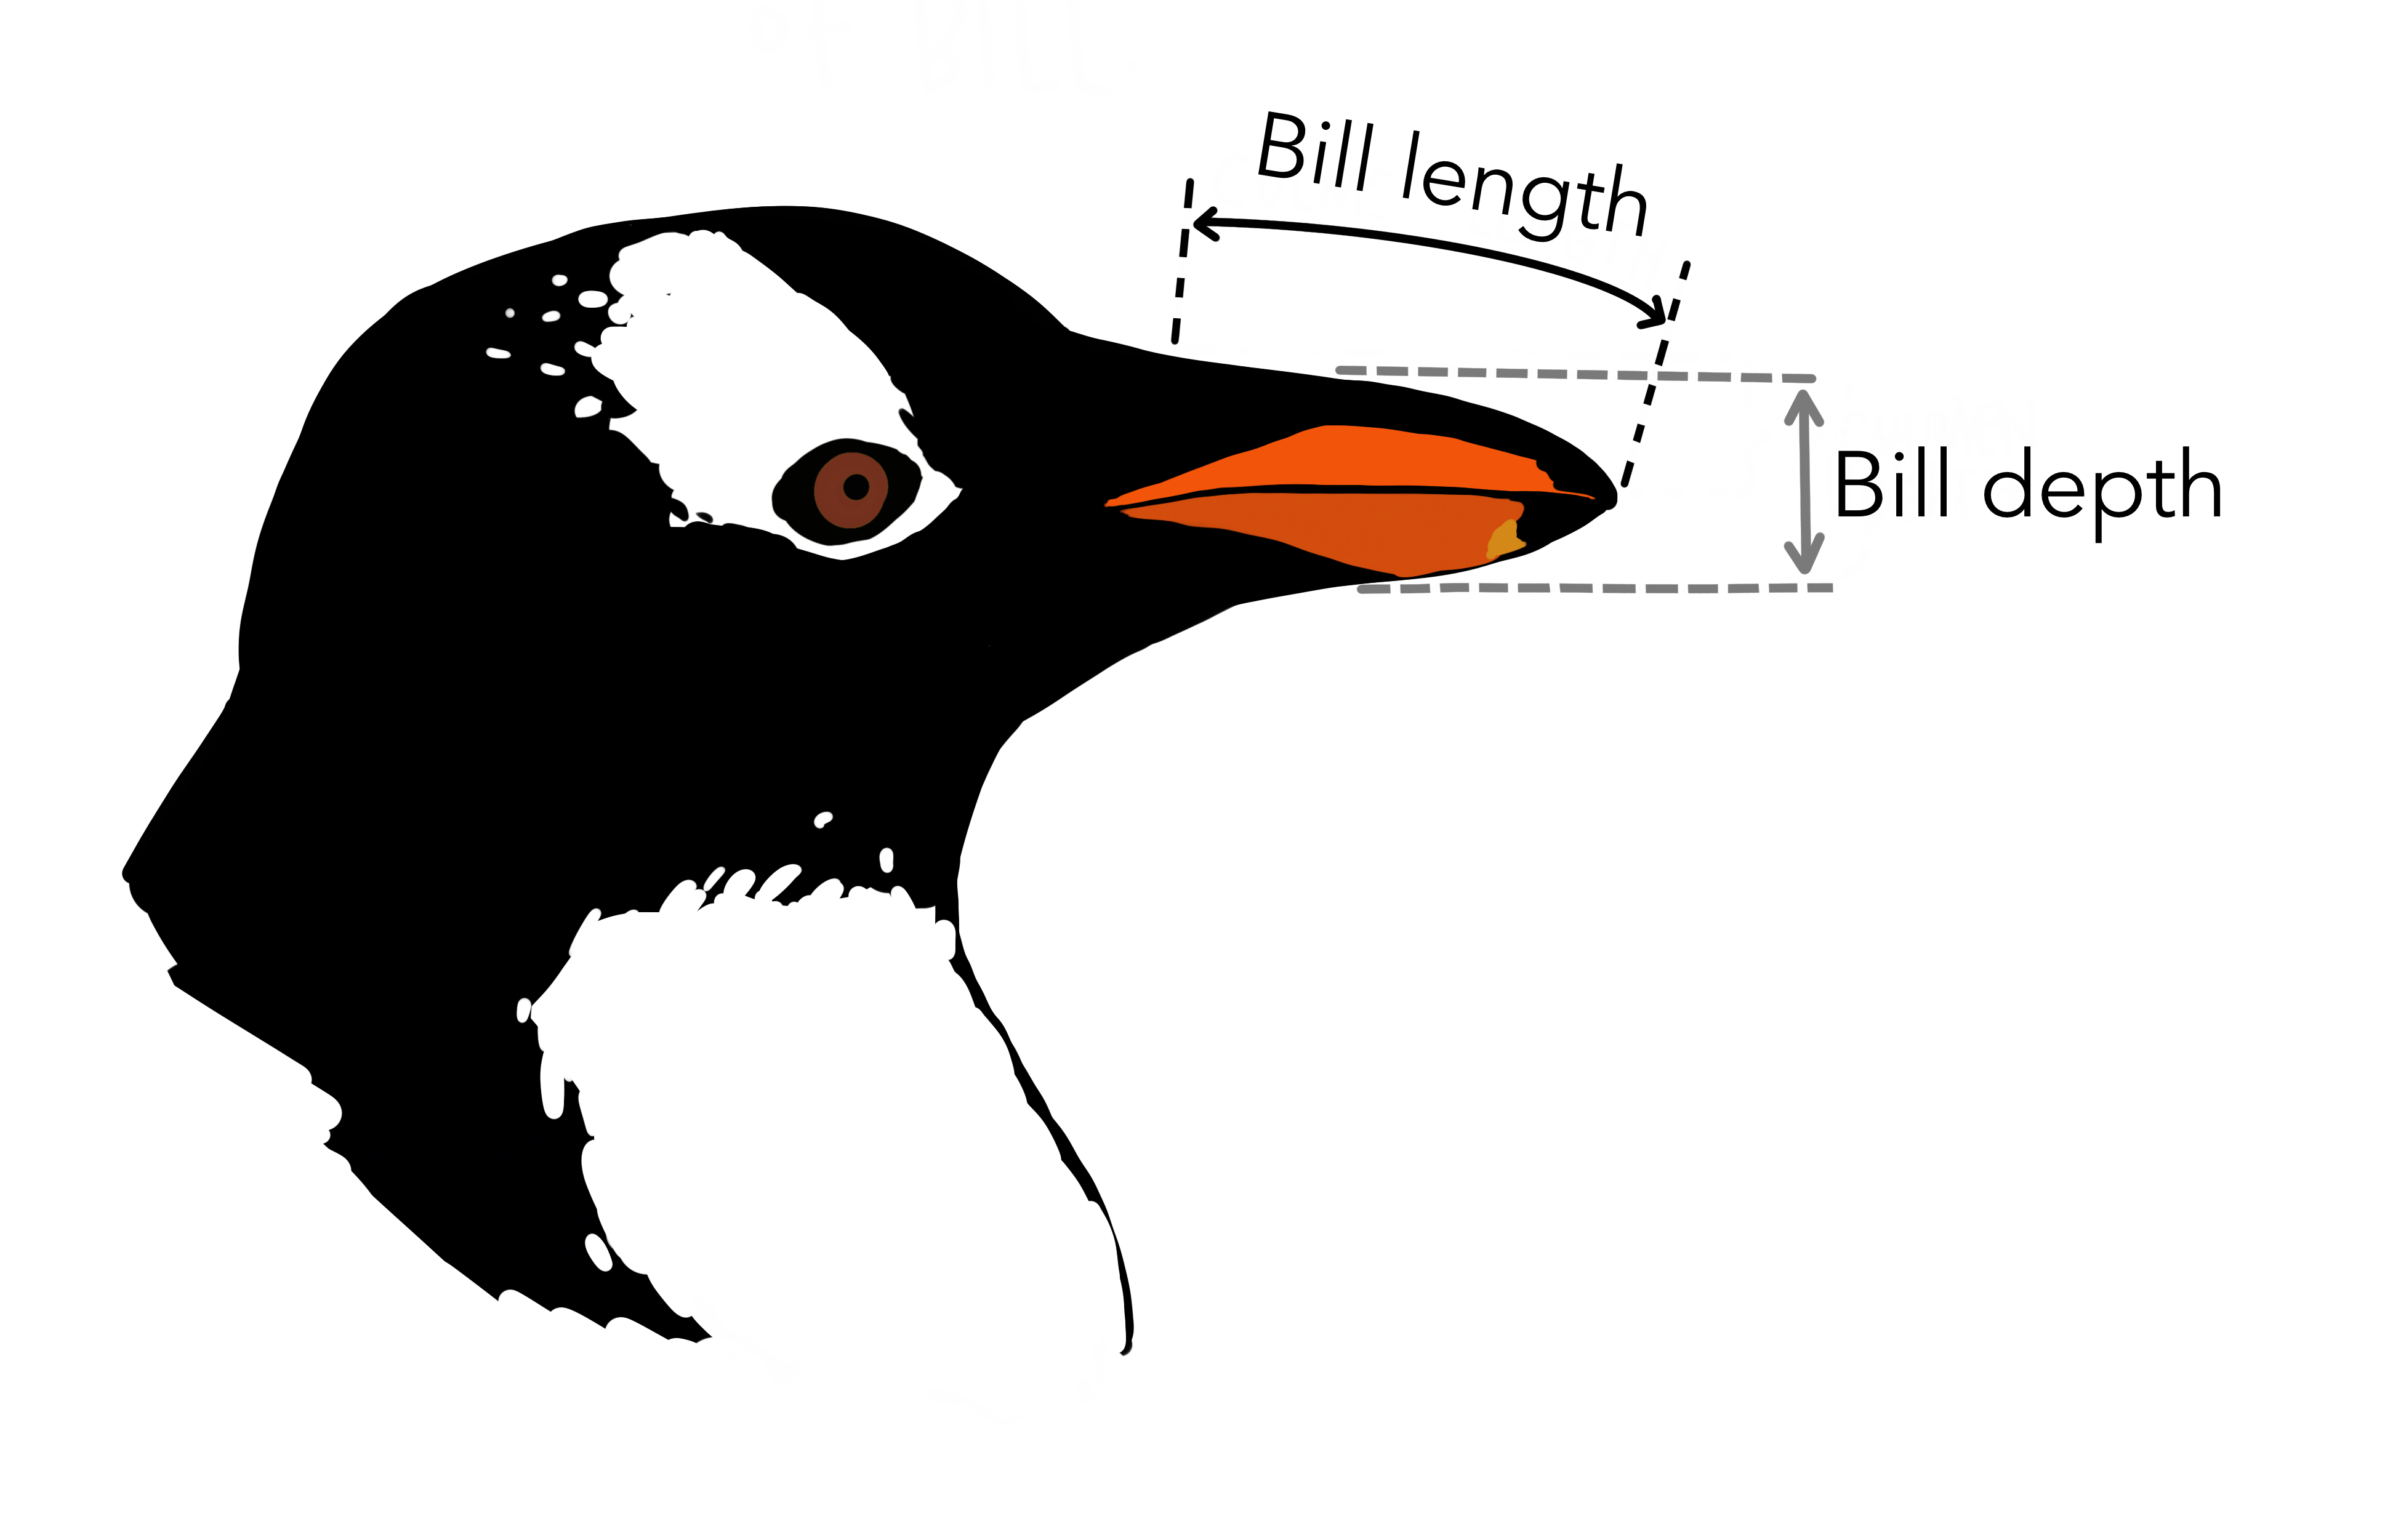
\includegraphics[width=5.20833in,height=\textheight]{chapters/../img/culmen_depth.png}

}

\caption{Ilustración de las variables \texttt{bill\_length\_mm} y
\texttt{bill\_depth\_mm} (Artista @allison\_horst)}

\end{figure}

Volviendo a mirar la primera fila de nuestra hoja de datos

\begin{verbatim}
/home/eva/.local/lib/python3.10/site-packages/IPython/core/formatters.py:342: FutureWarning:

In future versions `DataFrame.to_latex` is expected to utilise the base implementation of `Styler.to_latex` for formatting and rendering. The arguments signature may therefore change. It is recommended instead to use `DataFrame.style.to_latex` which also contains additional functionality.
\end{verbatim}

\begin{tabular}{lllrrrrl}
\toprule
{} & species &     island &  bill\_length\_mm &  bill\_depth\_mm &  flipper\_length\_mm &  body\_mass\_g &   sex \\
\midrule
0 &  Adelie &  Torgersen &            39.1 &           18.7 &              181.0 &       3750.0 &  MALE \\
\bottomrule
\end{tabular}

ahora sabes que el primer pingüino es de la especie Adelie, vive en la
isla Torgensen, las dimensiones de su pico son \(39.1 \times 18.7\)
milímetros, sus alas miden \(181\) milímetros, pesa \(3750\) gramos, y
es una hembra.

\hypertarget{valores-nulos}{%
\subsection{Valores nulos}\label{valores-nulos}}

Fíjate ahora en la columna \texttt{Non-Null\ Count} de la salida del
método \texttt{info()}:

\begin{verbatim}
<class 'pandas.core.frame.DataFrame'>
RangeIndex: 344 entries, 0 to 343
Data columns (total 7 columns):
 #   Column             Non-Null Count  Dtype  
---  ------             --------------  -----  
 0   species            344 non-null    object 
 1   island             344 non-null    object 
 2   bill_length_mm     342 non-null    float64
 3   bill_depth_mm      342 non-null    float64
 4   flipper_length_mm  342 non-null    float64
 5   body_mass_g        342 non-null    float64
 6   sex                333 non-null    object 
dtypes: float64(4), object(3)
memory usage: 18.9+ KB
\end{verbatim}

\begin{itemize}
\tightlist
\item[$\square$]
  TODO
\end{itemize}

\hypertarget{tipos-de-variables}{%
\subsection{Tipos de variables}\label{tipos-de-variables}}

Fíjate ahora en la columna \texttt{Dtype} de la salida del método
\texttt{info()}:

\begin{verbatim}
<class 'pandas.core.frame.DataFrame'>
RangeIndex: 344 entries, 0 to 343
Data columns (total 7 columns):
 #   Column             Non-Null Count  Dtype  
---  ------             --------------  -----  
 0   species            344 non-null    object 
 1   island             344 non-null    object 
 2   bill_length_mm     342 non-null    float64
 3   bill_depth_mm      342 non-null    float64
 4   flipper_length_mm  342 non-null    float64
 5   body_mass_g        342 non-null    float64
 6   sex                333 non-null    object 
dtypes: float64(4), object(3)
memory usage: 18.9+ KB
\end{verbatim}

\begin{itemize}
\tightlist
\item[$\square$]
  Hay \texttt{dtype} y \texttt{dtypes}
\item[$\square$]
  Numéricas vs categóricas
\item[$\square$]
  ¿Hablar aquí de conversión a categórica (\texttt{astype("category")})?
\item[$\square$]
  Mirar si \texttt{describe} se comporta diferente para numerica,
  \texttt{object} y \texttt{category}.
\end{itemize}

\hypertarget{uxedndice-de-una-hoja-de-datos}{%
\subsection{Índice de una hoja de
datos}\label{uxedndice-de-una-hoja-de-datos}}

Igual que cada columna tiene un nombre, cada fila también tiene una
etiqueta identificativa. En nuestra hoja de datos cada uno de los
\(344\) pingüinos se identifica con un número entero de la secuencia 0,
1, \ldots, 333.

\begin{verbatim}
/home/eva/.local/lib/python3.10/site-packages/IPython/core/formatters.py:342: FutureWarning:

In future versions `DataFrame.to_latex` is expected to utilise the base implementation of `Styler.to_latex` for formatting and rendering. The arguments signature may therefore change. It is recommended instead to use `DataFrame.style.to_latex` which also contains additional functionality.
\end{verbatim}

\begin{tabular}{lllrrrrl}
\toprule
{} & species &     island &  bill\_length\_mm &  bill\_depth\_mm &  flipper\_length\_mm &  body\_mass\_g &     sex \\
\midrule
0 &  Adelie &  Torgersen &            39.1 &           18.7 &              181.0 &       3750.0 &    MALE \\
1 &  Adelie &  Torgersen &            39.5 &           17.4 &              186.0 &       3800.0 &  FEMALE \\
2 &  Adelie &  Torgersen &            40.3 &           18.0 &              195.0 &       3250.0 &  FEMALE \\
\bottomrule
\end{tabular}

\begin{verbatim}
/home/eva/.local/lib/python3.10/site-packages/IPython/core/formatters.py:342: FutureWarning:

In future versions `DataFrame.to_latex` is expected to utilise the base implementation of `Styler.to_latex` for formatting and rendering. The arguments signature may therefore change. It is recommended instead to use `DataFrame.style.to_latex` which also contains additional functionality.
\end{verbatim}

\begin{tabular}{lllrrrrl}
\toprule
{} & species &  island &  bill\_length\_mm &  bill\_depth\_mm &  flipper\_length\_mm &  body\_mass\_g &     sex \\
\midrule
341 &  Gentoo &  Biscoe &            50.4 &           15.7 &              222.0 &       5750.0 &    MALE \\
342 &  Gentoo &  Biscoe &            45.2 &           14.8 &              212.0 &       5200.0 &  FEMALE \\
343 &  Gentoo &  Biscoe &            49.9 &           16.1 &              213.0 &       5400.0 &    MALE \\
\bottomrule
\end{tabular}

Las etiquetas identificativas de las filas de una hoja de datos forman
su \textbf{índice}. El índice de una hoja de datos de \texttt{pandas} se
registra en su propiedad \texttt{index}.

\begin{Shaded}
\begin{Highlighting}[]
\NormalTok{penguins.index}
\end{Highlighting}
\end{Shaded}

\begin{verbatim}
RangeIndex(start=0, stop=344, step=1)
\end{verbatim}

Si cada pingüino estuviera identificado por un código, podríamos haber
indicado utilizar esa variable como índice en el momento de la
importación de los datos. Cuando no se indica el índice de una hoja de
datos de forma explícita, \texttt{pandas} asigna una secuencia de
números enteros comenzando en 0, como ha ocurrido en nuestro caso.

\begin{exercise}[]% 
\protect\hypertarget{exr-data}{}\label{exr-data}%
Describe las características del tercer pingüino del estudio (índice 2).

\end{exercise}

\bookmarksetup{startatroot}

\hypertarget{una-variable-categuxf3rica}{%
\section{Una variable categórica}\label{una-variable-categuxf3rica}}

\hypertarget{el-muxe9todo-describe}{%
\subsection{\texorpdfstring{El método
\texttt{describe()}}{El método describe()}}\label{el-muxe9todo-describe}}

\begin{Shaded}
\begin{Highlighting}[]
\NormalTok{species }\OperatorTok{=}\NormalTok{ penguins[[}\StringTok{"species"}\NormalTok{]]}
\end{Highlighting}
\end{Shaded}

\begin{Shaded}
\begin{Highlighting}[]
\NormalTok{species.describe()}
\end{Highlighting}
\end{Shaded}

\begin{verbatim}
C:\Users\Usuario\AppData\Local\Programs\Python\Python310\lib\site-packages\IPython\core\formatters.py:343: FutureWarning:

In future versions `DataFrame.to_latex` is expected to utilise the base implementation of `Styler.to_latex` for formatting and rendering. The arguments signature may therefore change. It is recommended instead to use `DataFrame.style.to_latex` which also contains additional functionality.
\end{verbatim}

\begin{tabular}{ll}
\toprule
{} & species \\
\midrule
count  &     344 \\
unique &       3 \\
top    &  Adelie \\
freq   &     152 \\
\bottomrule
\end{tabular}

\begin{itemize}
\item[$\square$]
  Decir las funciones individuales.
\item[$\square$]
  ¿Hay diferencia entre convertirla a categórica
  (\texttt{astype("category")}) o no ?
\end{itemize}

\hypertarget{tabla-de-frecuencias}{%
\subsection{Tabla de frecuencias}\label{tabla-de-frecuencias}}

Tabla de frecuencias absolutas:

\begin{Shaded}
\begin{Highlighting}[]
\NormalTok{species\_counts }\OperatorTok{=}\NormalTok{ penguins.value\_counts(subset}\OperatorTok{=}\StringTok{"species"}\NormalTok{)}
\NormalTok{species\_counts}
\end{Highlighting}
\end{Shaded}

\begin{verbatim}
C:\Users\Usuario\AppData\Local\Programs\Python\Python310\lib\site-packages\IPython\core\formatters.py:343: FutureWarning:

In future versions `DataFrame.to_latex` is expected to utilise the base implementation of `Styler.to_latex` for formatting and rendering. The arguments signature may therefore change. It is recommended instead to use `DataFrame.style.to_latex` which also contains additional functionality.
\end{verbatim}

\begin{tabular}{lr}
\toprule
{} &    0 \\
species   &      \\
\midrule
Adelie    &  152 \\
Gentoo    &  124 \\
Chinstrap &   68 \\
\bottomrule
\end{tabular}

\begin{Shaded}
\begin{Highlighting}[]
\BuiltInTok{type}\NormalTok{(species\_counts)}
\end{Highlighting}
\end{Shaded}

\begin{verbatim}
pandas.core.series.Series
\end{verbatim}

\begin{Shaded}
\begin{Highlighting}[]
\NormalTok{species\_counts.index}
\end{Highlighting}
\end{Shaded}

\begin{verbatim}
Index(['Adelie', 'Gentoo', 'Chinstrap'], dtype='object', name='species')
\end{verbatim}

\begin{exercise}[]% 
\protect\hypertarget{exr-1categorial-sex-counts}{}\label{exr-1categorial-sex-counts}%
Determina el número total de hembras y de machos. Almacena el resultado
en una variable de nombre \texttt{sex\_counts}.

\end{exercise}

Tabla de frecuencias relativas (proporciones):

\begin{Shaded}
\begin{Highlighting}[]
\NormalTok{species\_props }\OperatorTok{=}\NormalTok{ penguins.value\_counts(}
\NormalTok{    subset}\OperatorTok{=}\StringTok{"species"}\NormalTok{,}
\NormalTok{    normalize}\OperatorTok{=}\VariableTok{True}
\NormalTok{)}
\NormalTok{species\_props}
\end{Highlighting}
\end{Shaded}

\begin{verbatim}
C:\Users\Usuario\AppData\Local\Programs\Python\Python310\lib\site-packages\IPython\core\formatters.py:343: FutureWarning:

In future versions `DataFrame.to_latex` is expected to utilise the base implementation of `Styler.to_latex` for formatting and rendering. The arguments signature may therefore change. It is recommended instead to use `DataFrame.style.to_latex` which also contains additional functionality.
\end{verbatim}

\begin{tabular}{lr}
\toprule
{} &         0 \\
species   &           \\
\midrule
Adelie    &  0.441860 \\
Gentoo    &  0.360465 \\
Chinstrap &  0.197674 \\
\bottomrule
\end{tabular}

Tabla de porcentajes:

\begin{Shaded}
\begin{Highlighting}[]
\DecValTok{100}\OperatorTok{*}\NormalTok{species\_props}
\end{Highlighting}
\end{Shaded}

\begin{tabular}{lr}
\toprule
{} &          0 \\
species   &            \\
\midrule
Adelie    &  44.186047 \\
Gentoo    &  36.046512 \\
Chinstrap &  19.767442 \\
\bottomrule
\end{tabular}

\hypertarget{diagrama-de-barras-con-pandas}{%
\subsection{\texorpdfstring{Diagrama de barras con
\texttt{pandas}}{Diagrama de barras con pandas}}\label{diagrama-de-barras-con-pandas}}

\begin{Shaded}
\begin{Highlighting}[]
\NormalTok{species\_counts.plot.bar()}\OperatorTok{;}
\end{Highlighting}
\end{Shaded}

\begin{figure}[tbph]

{\centering 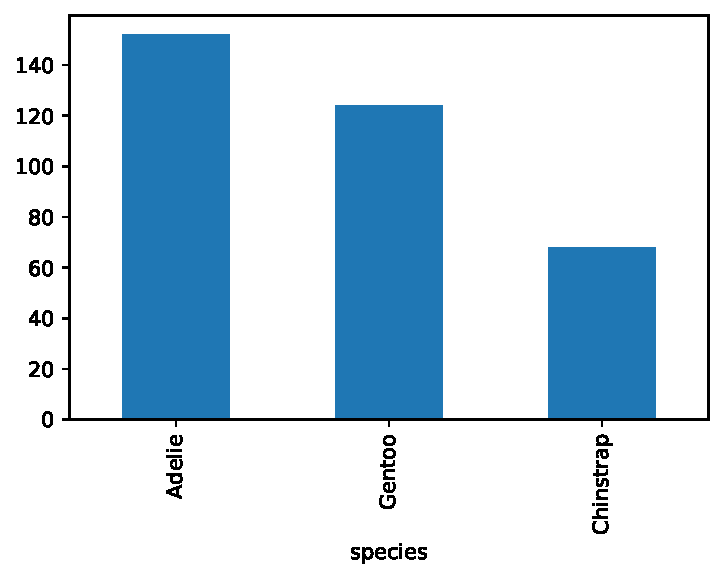
\includegraphics{chapters/1categorical_files/figure-pdf/cell-10-output-1.pdf}

}

\end{figure}

\begin{Shaded}
\begin{Highlighting}[]
\NormalTok{species\_counts.plot.barh()}\OperatorTok{;}
\end{Highlighting}
\end{Shaded}

\begin{figure}[tbph]

{\centering 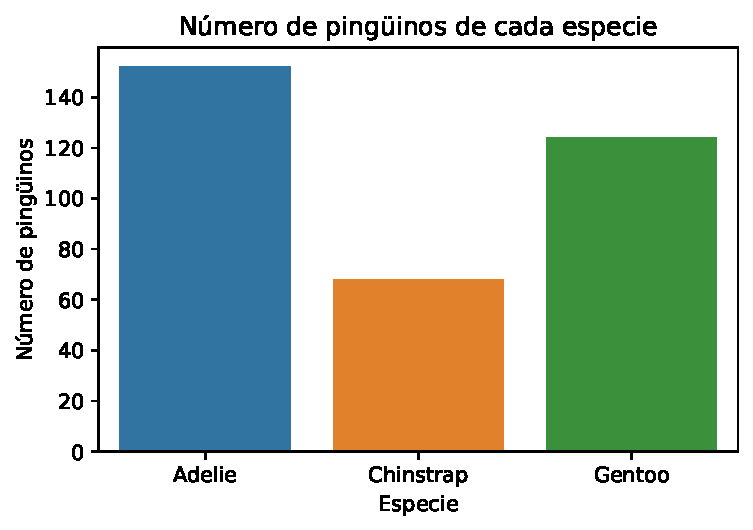
\includegraphics{chapters/1categorical_files/figure-pdf/cell-11-output-1.pdf}

}

\end{figure}

\begin{exercise}[]% 
\protect\hypertarget{exr-1categorial-pd-sex-bar}{}\label{exr-1categorial-pd-sex-bar}%
Usa la variable \texttt{sex\_counts} creada en el
\exrref{exr-1categorial-sex-counts} para crear un diagrama de
barras mostrando el número total de hembras y de machos.

\end{exercise}

\begin{exercise}[]% 
\protect\hypertarget{exr-1categorial-pd-island}{}\label{exr-1categorial-pd-island}%
Determina cuántos pingüinos hay en cada isla y dibuja un diagrama de
barras con los resultados.

\end{exercise}

\hypertarget{diagrama-de-barras-con-seaborn}{%
\subsection{\texorpdfstring{Diagrama de barras con
\texttt{seaborn}}{Diagrama de barras con seaborn}}\label{diagrama-de-barras-con-seaborn}}

\begin{Shaded}
\begin{Highlighting}[]
\NormalTok{sns.barplot(x}\OperatorTok{=}\NormalTok{species\_counts.index, y}\OperatorTok{=}\NormalTok{species\_counts)}\OperatorTok{;}
\end{Highlighting}
\end{Shaded}

\begin{figure}[tbph]

{\centering 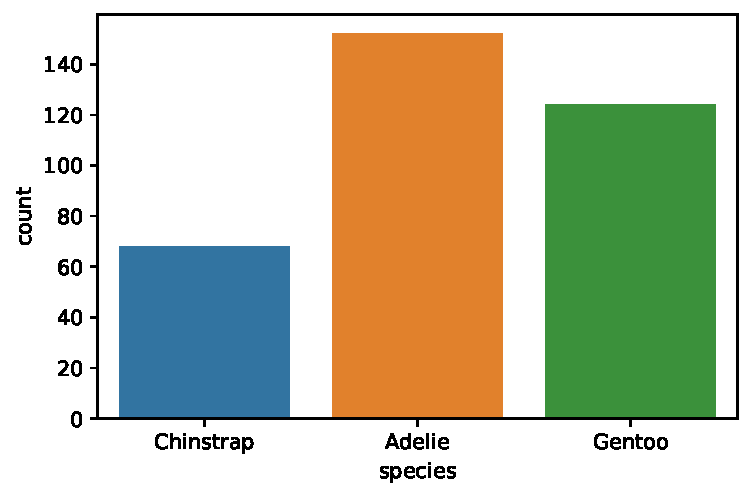
\includegraphics{chapters/1categorical_files/figure-pdf/cell-12-output-1.pdf}

}

\end{figure}

\begin{Shaded}
\begin{Highlighting}[]
\NormalTok{sns.countplot(data}\OperatorTok{=}\NormalTok{penguins, x}\OperatorTok{=}\StringTok{"species"}\NormalTok{)}\OperatorTok{;}
\end{Highlighting}
\end{Shaded}

\begin{figure}[tbph]

{\centering 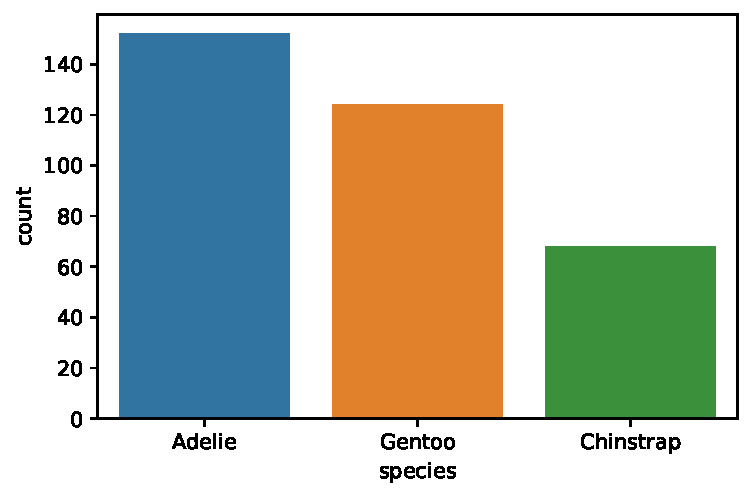
\includegraphics{chapters/1categorical_files/figure-pdf/cell-13-output-1.pdf}

}

\end{figure}

\begin{Shaded}
\begin{Highlighting}[]
\NormalTok{sns.countplot(data}\OperatorTok{=}\NormalTok{penguins, x}\OperatorTok{=}\StringTok{"species"}\NormalTok{, order }\OperatorTok{=}\NormalTok{ [}\StringTok{\textquotesingle{}Chinstrap\textquotesingle{}}\NormalTok{, }\StringTok{\textquotesingle{}Adelie\textquotesingle{}}\NormalTok{, }\StringTok{\textquotesingle{}Gentoo\textquotesingle{}}\NormalTok{])}\OperatorTok{;}
\end{Highlighting}
\end{Shaded}

\begin{figure}[tbph]

{\centering 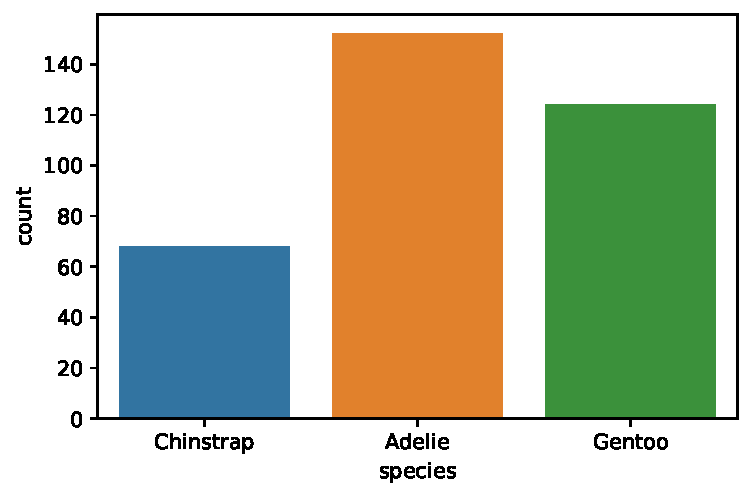
\includegraphics{chapters/1categorical_files/figure-pdf/cell-14-output-1.pdf}

}

\end{figure}

\begin{Shaded}
\begin{Highlighting}[]
\NormalTok{sns.countplot(data}\OperatorTok{=}\NormalTok{penguins, x}\OperatorTok{=}\StringTok{"species"}\NormalTok{, order }\OperatorTok{=}\NormalTok{ species\_counts.index)}\OperatorTok{;}
\end{Highlighting}
\end{Shaded}

\begin{figure}[tbph]

{\centering 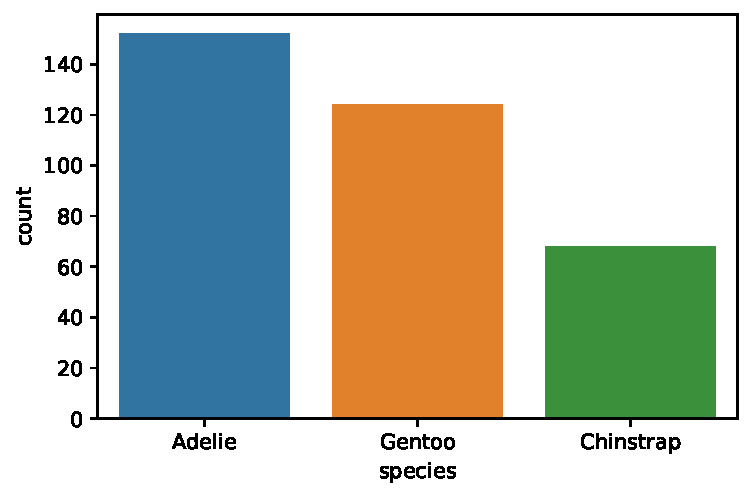
\includegraphics{chapters/1categorical_files/figure-pdf/cell-15-output-1.pdf}

}

\end{figure}

\begin{Shaded}
\begin{Highlighting}[]
\NormalTok{sns.countplot(data}\OperatorTok{=}\NormalTok{penguins, y}\OperatorTok{=}\StringTok{"species"}\NormalTok{)}\OperatorTok{;}
\end{Highlighting}
\end{Shaded}

\begin{figure}[tbph]

{\centering 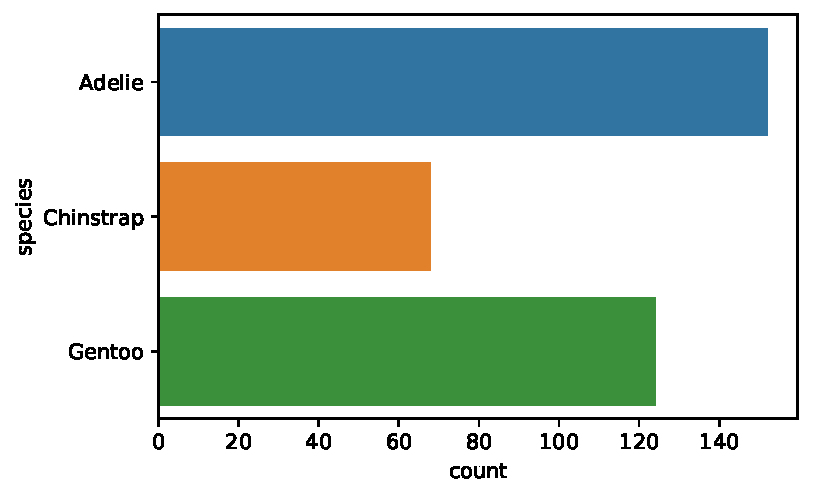
\includegraphics{chapters/1categorical_files/figure-pdf/cell-16-output-1.pdf}

}

\end{figure}

\begin{exercise}[]% 
\protect\hypertarget{exr-1categorial-sns-countplot}{}\label{exr-1categorial-sns-countplot}%
Utiliza la función \VERB|\NormalTok{countplot()}| de la librería
\VERB|\NormalTok{seaborn}| para crear diagramas de barras para

\begin{itemize}
\tightlist
\item
  el número de hembras y machos
\item
  el número de pingüinos en cada isla
\end{itemize}

sin crear previamente tablas de recuentos.

\end{exercise}

\hypertarget{personalizaciuxf3n-de-los-gruxe1ficos}{%
\subsubsection{Personalización de los
gráficos}\label{personalizaciuxf3n-de-los-gruxe1ficos}}

No es difícil personalizar los gráficos indicando títulos y colores
\footnote{Puedes ver los colores disponibles
  \href{https://matplotlib.org/stable/tutorials/colors/colors.html}{aquí}.}.
Por ejemplo:

\begin{Shaded}
\begin{Highlighting}[]
\NormalTok{sns.countplot(data}\OperatorTok{=}\NormalTok{penguins, x}\OperatorTok{=}\StringTok{"species"}\NormalTok{, color}\OperatorTok{=}\StringTok{"steelblue"}\NormalTok{)}\OperatorTok{;}
\end{Highlighting}
\end{Shaded}

\begin{figure}[tbph]

{\centering 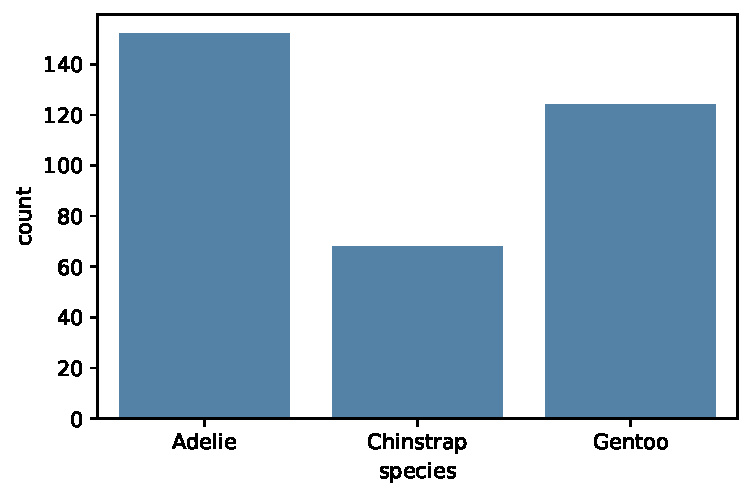
\includegraphics{chapters/1categorical_files/figure-pdf/cell-17-output-1.pdf}

}

\end{figure}

\begin{Shaded}
\begin{Highlighting}[]
\NormalTok{sns.countplot(data}\OperatorTok{=}\NormalTok{penguins, x}\OperatorTok{=}\StringTok{"species"}\NormalTok{, palette}\OperatorTok{=}\NormalTok{[}\StringTok{"steelblue"}\NormalTok{, }\StringTok{"coral"}\NormalTok{, }\StringTok{"gold"}\NormalTok{])}\OperatorTok{;}
\end{Highlighting}
\end{Shaded}

\begin{figure}[tbph]

{\centering 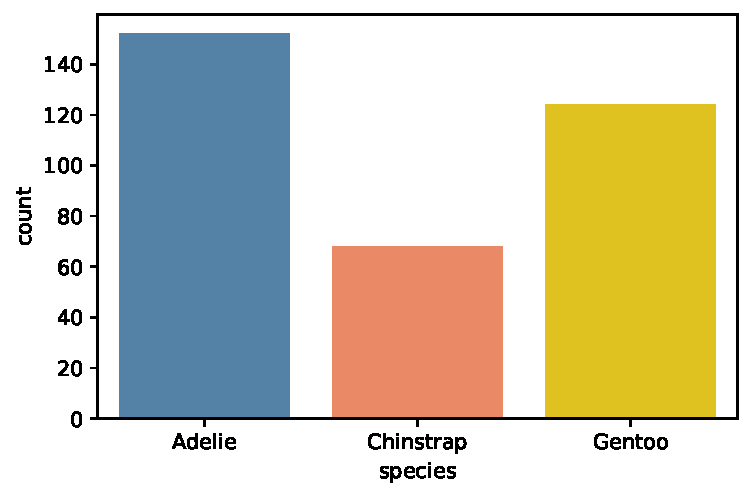
\includegraphics{chapters/1categorical_files/figure-pdf/cell-18-output-1.pdf}

}

\end{figure}

\begin{Shaded}
\begin{Highlighting}[]
\NormalTok{ax }\OperatorTok{=}\NormalTok{ sns.countplot(data}\OperatorTok{=}\NormalTok{penguins, x}\OperatorTok{=}\StringTok{"species"}\NormalTok{, palette}\OperatorTok{=}\StringTok{"pastel"}\NormalTok{)}
\NormalTok{ax.}\BuiltInTok{set}\NormalTok{(}
\NormalTok{    title}\OperatorTok{=}\StringTok{"Número de pingüinos de cada especie"}\NormalTok{,}
\NormalTok{    xlabel}\OperatorTok{=}\StringTok{"Especie"}\NormalTok{, }
\NormalTok{    ylabel}\OperatorTok{=}\StringTok{"Número de pingüinos"}
\NormalTok{)}\OperatorTok{;}
\end{Highlighting}
\end{Shaded}

\begin{figure}[tbph]

{\centering 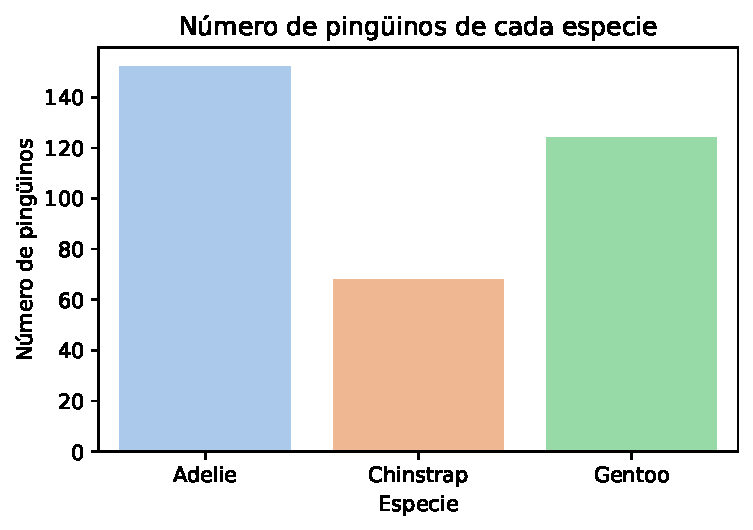
\includegraphics{chapters/1categorical_files/figure-pdf/cell-19-output-1.pdf}

}

\end{figure}

La personalización de los gráficos no carece de importancia, siendo
especialmente relevante dar títulos descriptivos a los ejes. No
obstante, en esta práctica nos centraremos en los procedimientos para
realizar los gráficos y en la mayoría de ocasiones omitiremos los
detalles de personalización de los mismos, que pueden consultarse en la
documentación de las librerías usadas.

\bookmarksetup{startatroot}

\hypertarget{una-variable-numuxe9rica}{%
\section{Una variable numérica}\label{una-variable-numuxe9rica}}

\hypertarget{el-muxe9todo-describe-1}{%
\subsection{\texorpdfstring{El método
\texttt{describe()}}{El método describe()}}\label{el-muxe9todo-describe-1}}

\hypertarget{histograma}{%
\subsection{Histograma}\label{histograma}}

\begin{itemize}
\tightlist
\item[$\square$]
  Están \texttt{Dataframe.plot.hist()} y \texttt{Dataframe.hist()}
\end{itemize}

\hypertarget{diagrama-de-caja-y-bigotes}{%
\subsection{Diagrama de caja y
bigotes}\label{diagrama-de-caja-y-bigotes}}

\begin{itemize}
\tightlist
\item[$\square$]
  Están \texttt{Dataframe.plot.box()} y \texttt{Dataframe.boxplot()}
\end{itemize}

\bookmarksetup{startatroot}

\hypertarget{agrupaciuxf3n-de-hojas-de-datos}{%
\section{Agrupación de hojas de
datos}\label{agrupaciuxf3n-de-hojas-de-datos}}

\begin{itemize}
\tightlist
\item[$\square$]
  Habiendo descubierto el argumento \texttt{subset} de
  \texttt{value\_counts()} y el método \texttt{unstack()} (ver en mis
  apuntes de pandas
  \texttt{Gráficos\ \textgreater{}\ Diagramas\ de\ barras\ \textgreater{}\ Dos\ variables}
  y
  \texttt{Gráficos\ \textgreater{}\ Diagramas\ de\ barras\ \textgreater{}\ Tres\ variables})
  puede que esta sección no haga falta hasta analizar variable numérica
  por categorías.
\end{itemize}

\begin{itemize}
\tightlist
\item
  Split
\item
  Apply
\item
  Combine
\end{itemize}

Un ejemplo sencillo como aplicar \texttt{sum()}.

O también tamaño muestral:

\begin{verbatim}
df.groupby("grade3").size()
\end{verbatim}

\bookmarksetup{startatroot}

\hypertarget{dos-variables-categuxf3ricas}{%
\section{Dos variables categóricas}\label{dos-variables-categuxf3ricas}}

\begin{itemize}
\tightlist
\item[$\square$]
  Ver lo que tengo explorado en mi manual de pandas en apartados
  \texttt{Gráficos\ \textgreater{}\ Diagramas\ de\ barras\ \textgreater{}\ Dos\ variables}
  y
  \texttt{Gráficos\ \textgreater{}\ Diagramas\ de\ barras\ \textgreater{}\ Tres\ variables}.
\end{itemize}

\hypertarget{tablas-de-frecuencias}{%
\subsection{Tablas de frecuencias}\label{tablas-de-frecuencias}}

\hypertarget{tablas-de-contingencia}{%
\subsection{Tablas de contingencia}\label{tablas-de-contingencia}}

\begin{verbatim}
pd.crosstab(df2["factor1"], df2["factor2"])
\end{verbatim}

\begin{verbatim}
pd.crosstab(
    df2["factor1"], 
    [df2["factor2"], df2["factor3"]]
)
\end{verbatim}

\bookmarksetup{startatroot}

\hypertarget{variable-numuxe9rica-por-categoruxedas}{%
\section{Variable numérica por
categorías}\label{variable-numuxe9rica-por-categoruxedas}}

\bookmarksetup{startatroot}



\cleardoublepage
\printsols
\myprintbibliography[title=Bibliografía]


\end{document}
